\newpage
\section{Kết quả}

\subsection{Môi trường thử nghiệm}

Các thí nghiệm được thực hiện trên phần cứng thật trong môi trường mạng LAN nội bộ. Mục tiêu kiểm thử là xác nhận toàn bộ luồng chức năng từ cảm biến, hiển thị, web điều khiển đến giao tiếp liên thiết bị qua MQTT.

\begin{table}[h!]
\centering
\caption{Cấu hình môi trường kiểm thử}
\begin{tabular}{|l|l|}
\hline
\textbf{Thành phần} & \textbf{Thông tin} \\
\hline
Vi điều khiển chính & YoloUNO (ESP32-S3) \\
\hline
Vi điều khiển phụ & ESP32-S3 DevKitC-1 \\
\hline
Cảm biến & DHT20, PIR \\
\hline
Thiết bị chấp hành & LCD I2C, NeoPixel RGB, quạt PWM, buzzer 5V \\
\hline
Nền tảng phát triển & PlatformIO + Arduino framework \\
\hline
Truyền thông nội bộ & WiFi AP/AP+STA, Mosquitto local broker \\
\hline
Cloud dashboard & CoreIOT \\
\hline
\end{tabular}
\end{table}

\subsection{Kết quả triển khai phần cứng}

Hai node phần cứng được lắp ráp và vận hành độc lập trước khi tích hợp liên thông. Node chính (YoloUNO) đảm nhận đo đạc, hiển thị và web server; node phụ (DevKitC-1) đảm nhận cảnh báo còi trong tính năng mở rộng.

\begin{figure}[H]
    \centering
    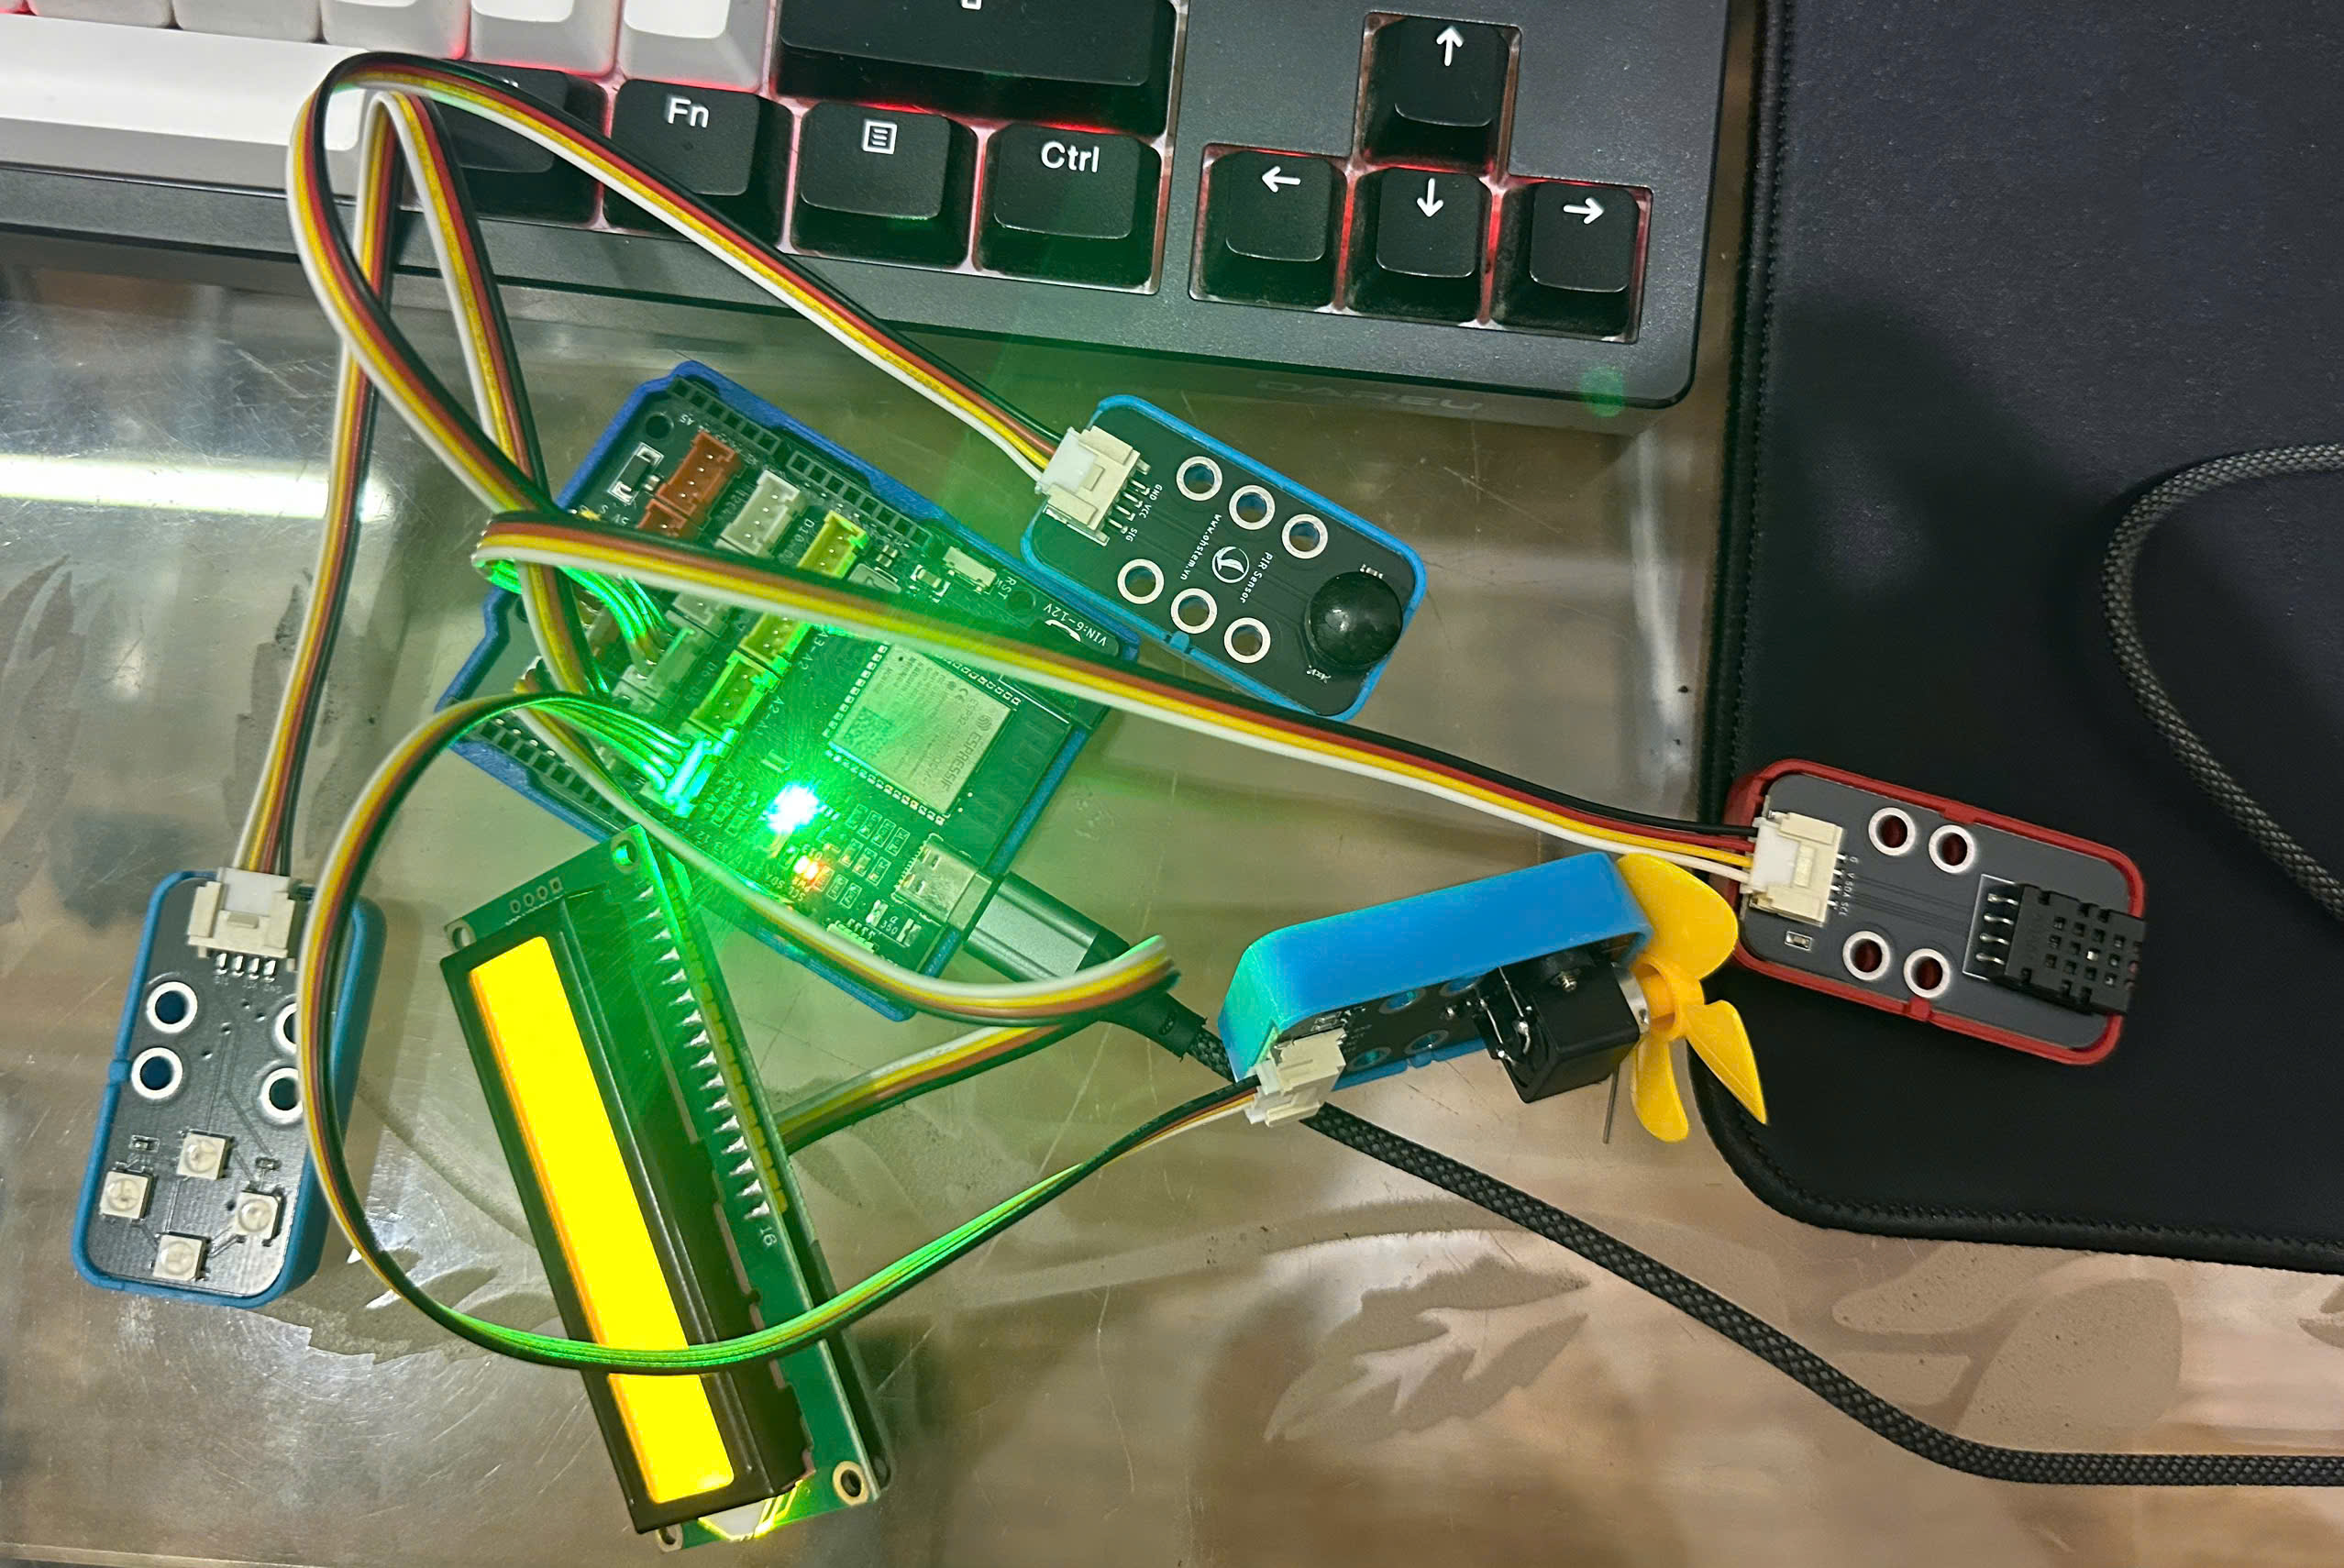
\includegraphics[width=1.1\textwidth]{pictures/res/yolo_uno.jpg}
    \caption{Kết nối phần cứng với YoloUNO}
\end{figure}

\begin{figure}[H]
    \centering
    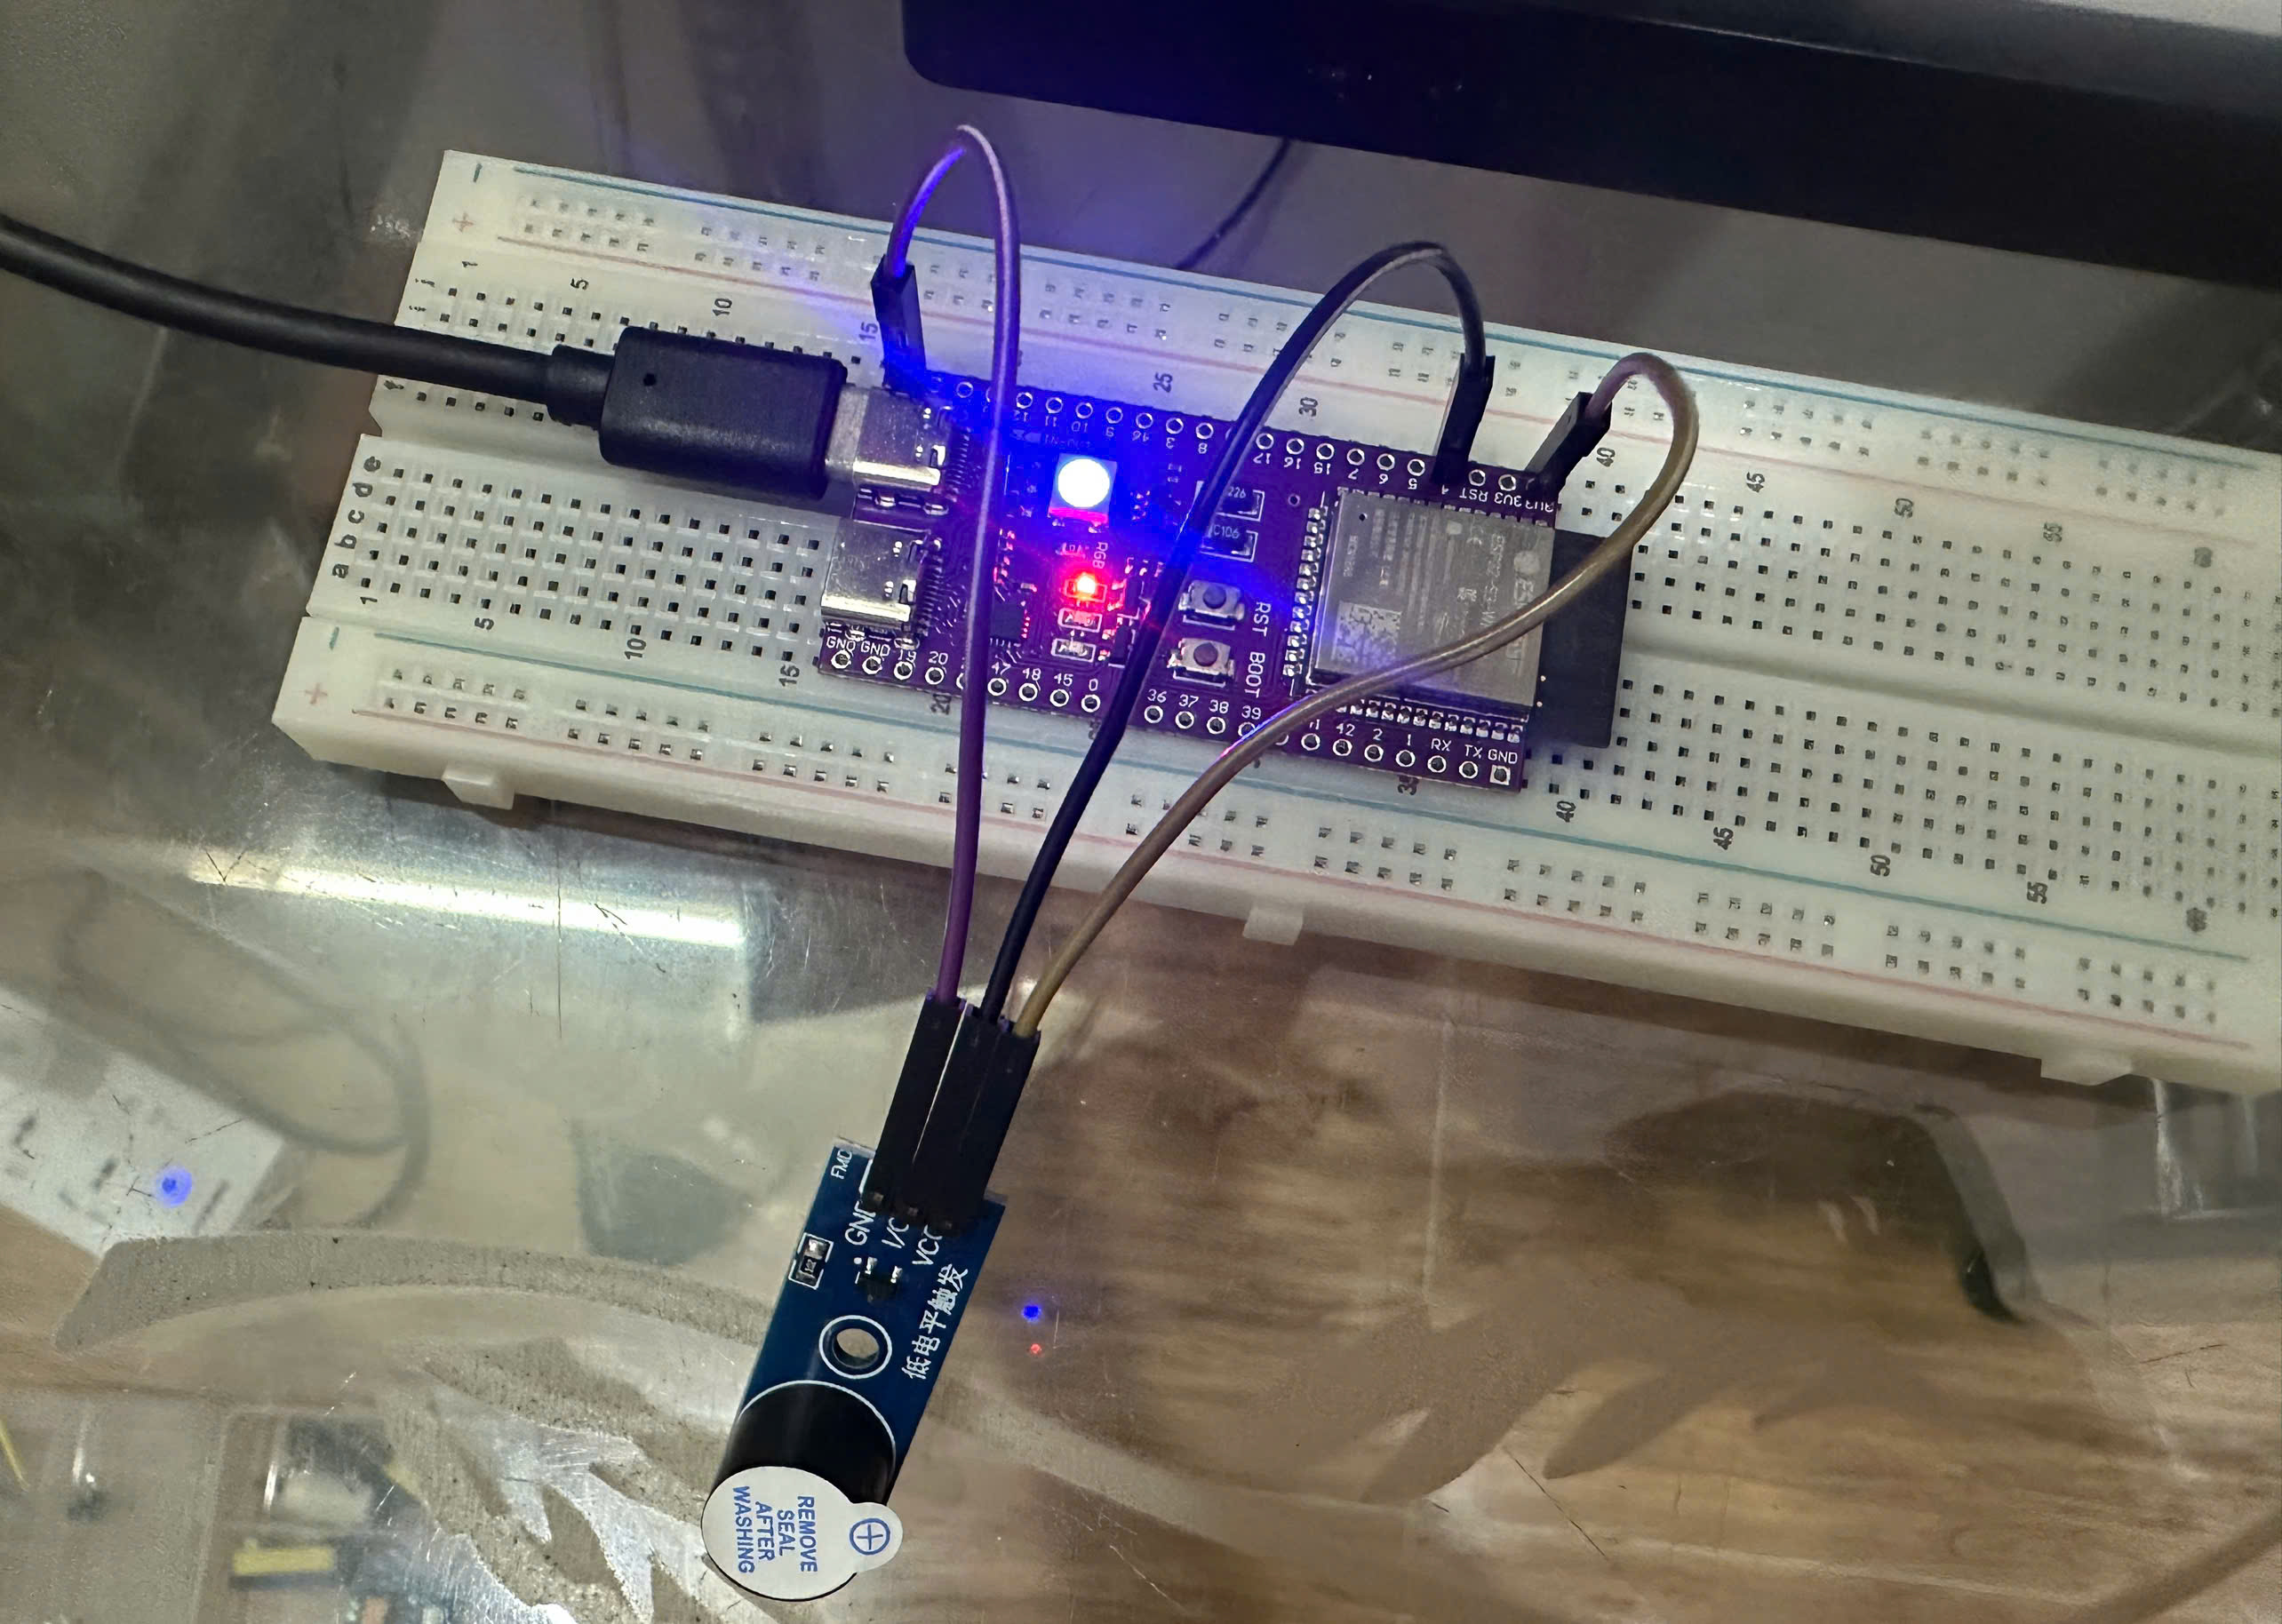
\includegraphics[width=1.1\textwidth]{pictures/res/devkitc1.jpg}
    \caption{Kết nối với ESP32-S3-DevKit-C1}
\end{figure}

Kết quả kiểm tra phần cứng cho thấy các chân tín hiệu hoạt động đúng theo cấu hình trong firmware: cảm biến đọc ổn định, LCD hiển thị đúng trạng thái, NeoPixel phản hồi điều khiển màu và quạt nhận PWM theo tốc độ cài đặt.

\subsection{Kết quả giao diện và giám sát}

Giao diện dashboard hiển thị được dữ liệu cảm biến theo thời gian thực và phản ánh trạng thái hệ thống để người dùng dễ quan sát. Trong các lần kiểm thử, dữ liệu gửi lên cloud và hiển thị trên dashboard CoreIOT đúng định dạng telemetry đã thiết kế.

\begin{figure}[H]
    \centering
    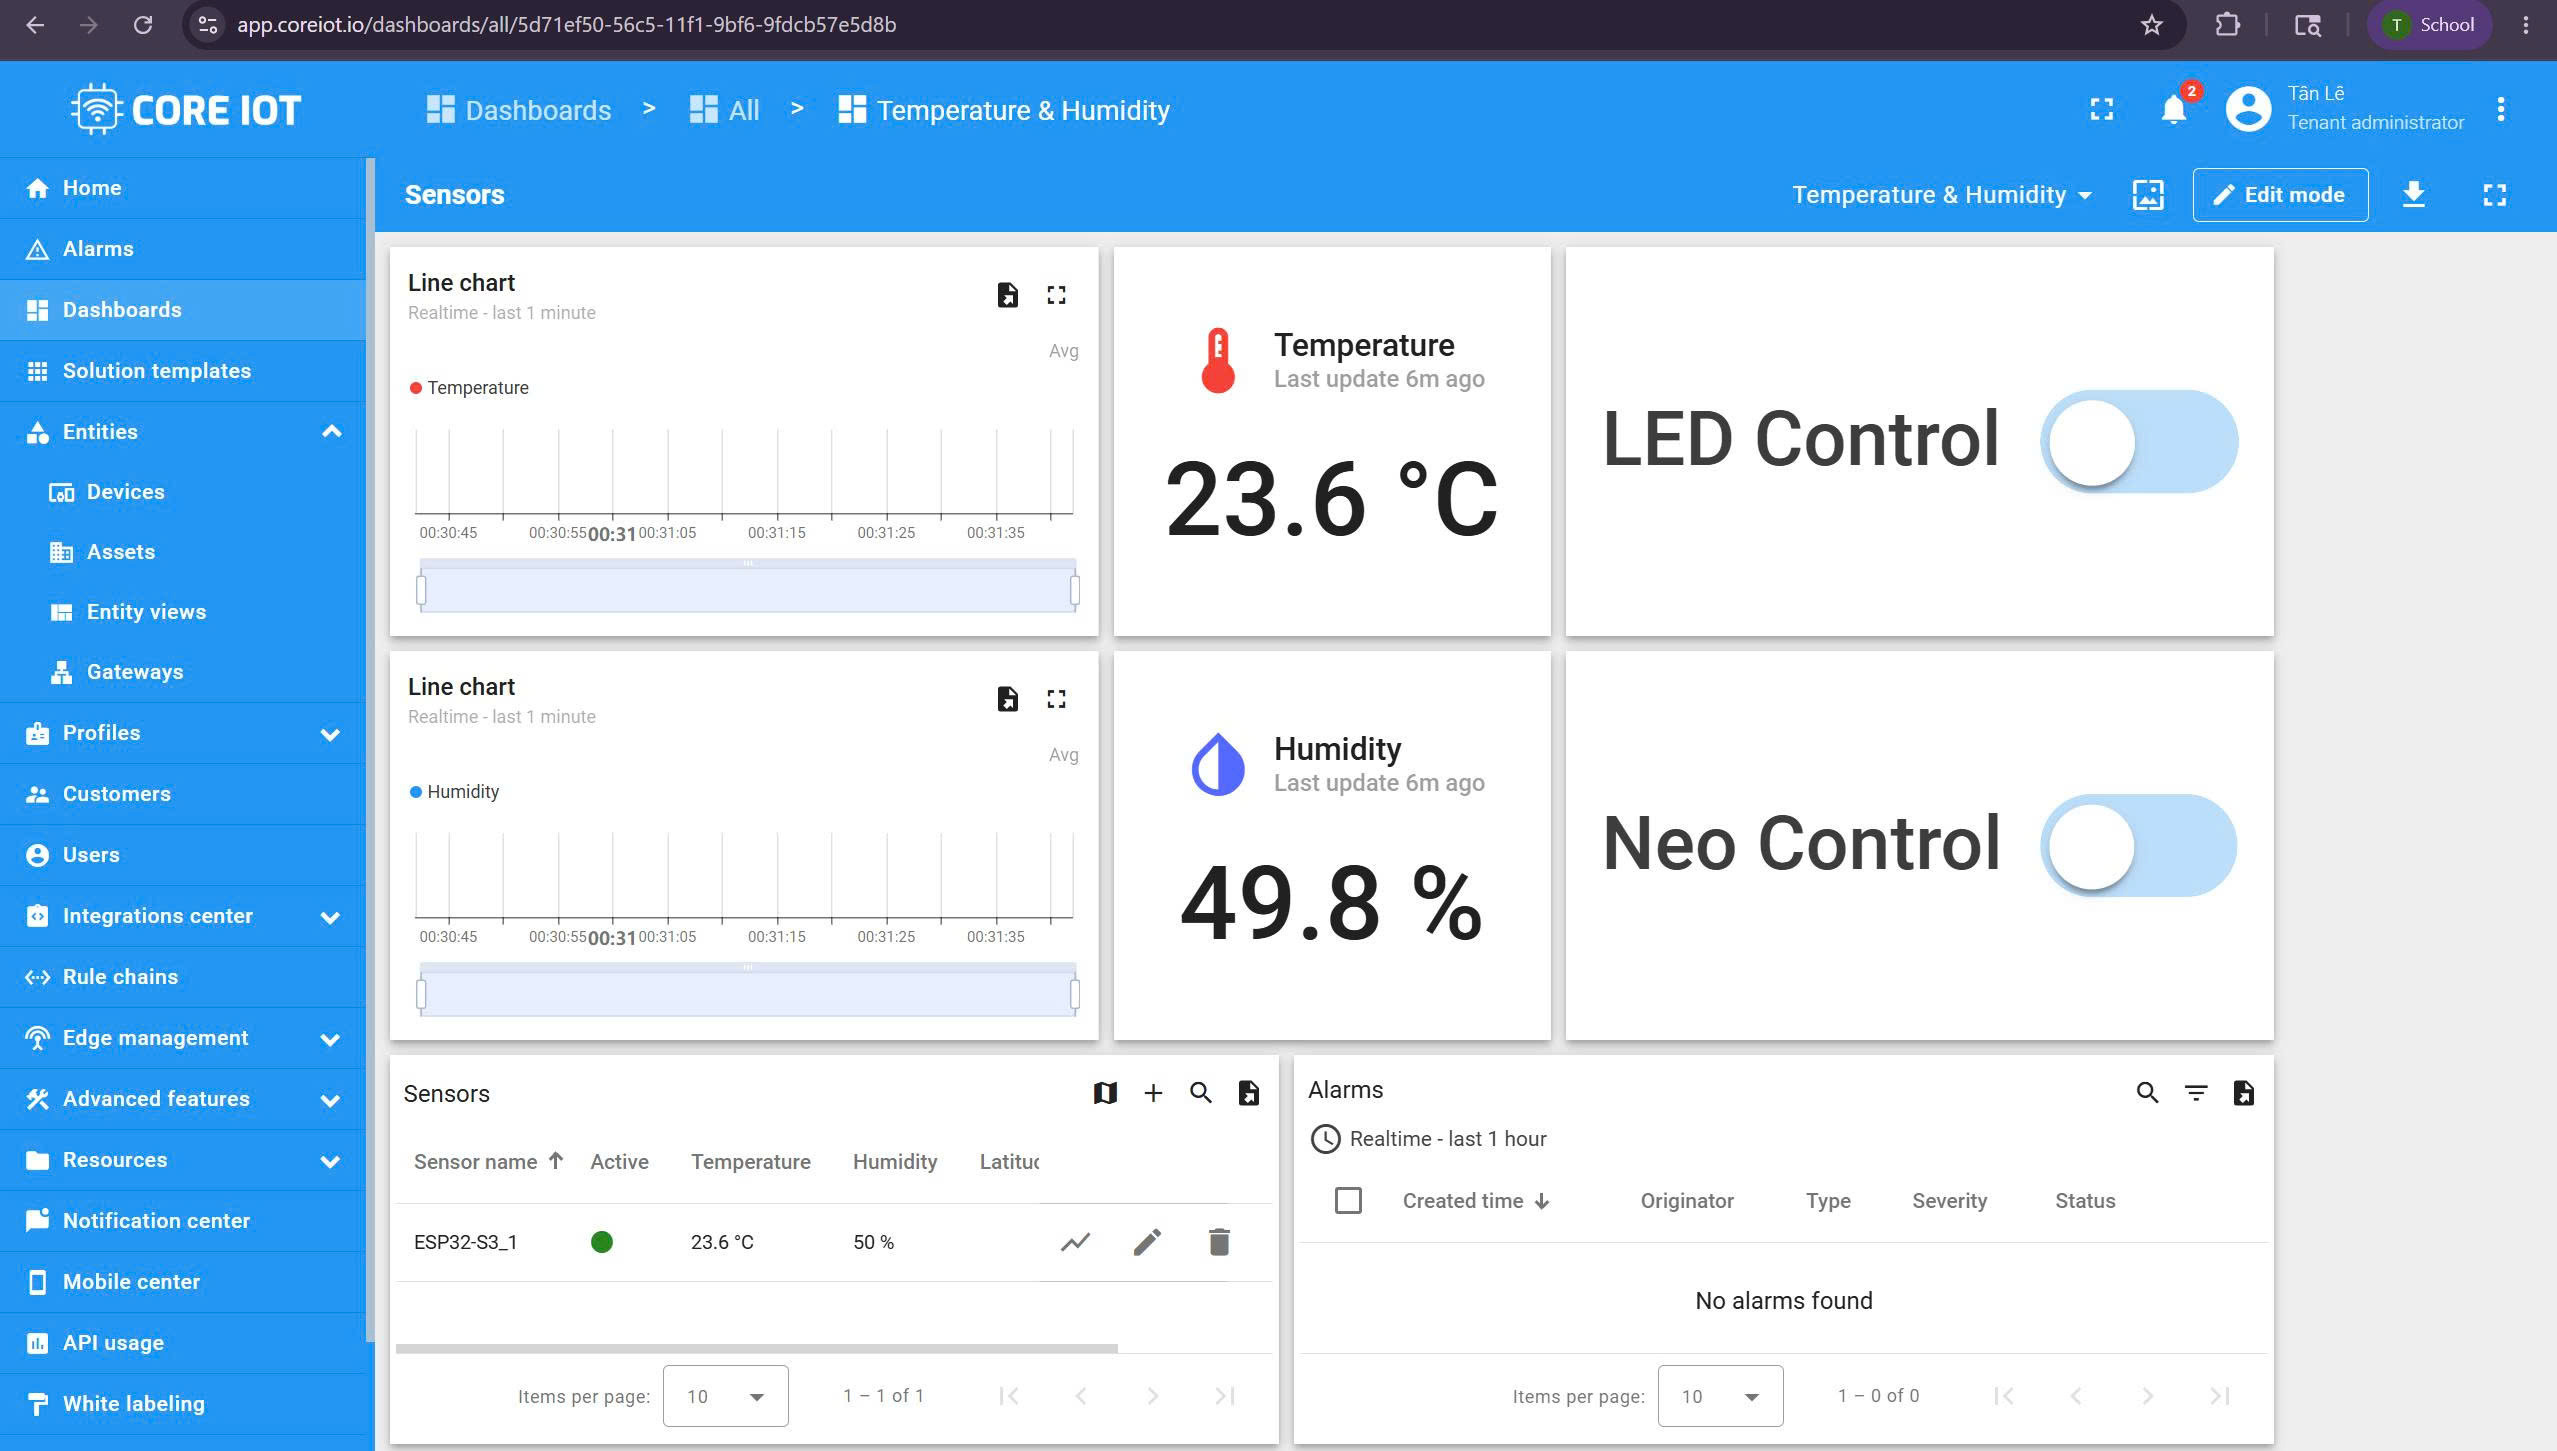
\includegraphics[width=1.1\textwidth]{pictures/res/dashboard.jpg}
    \caption{Dashboard trên server CoreIoT}
\end{figure}

\begin{figure}[H]
    \centering
    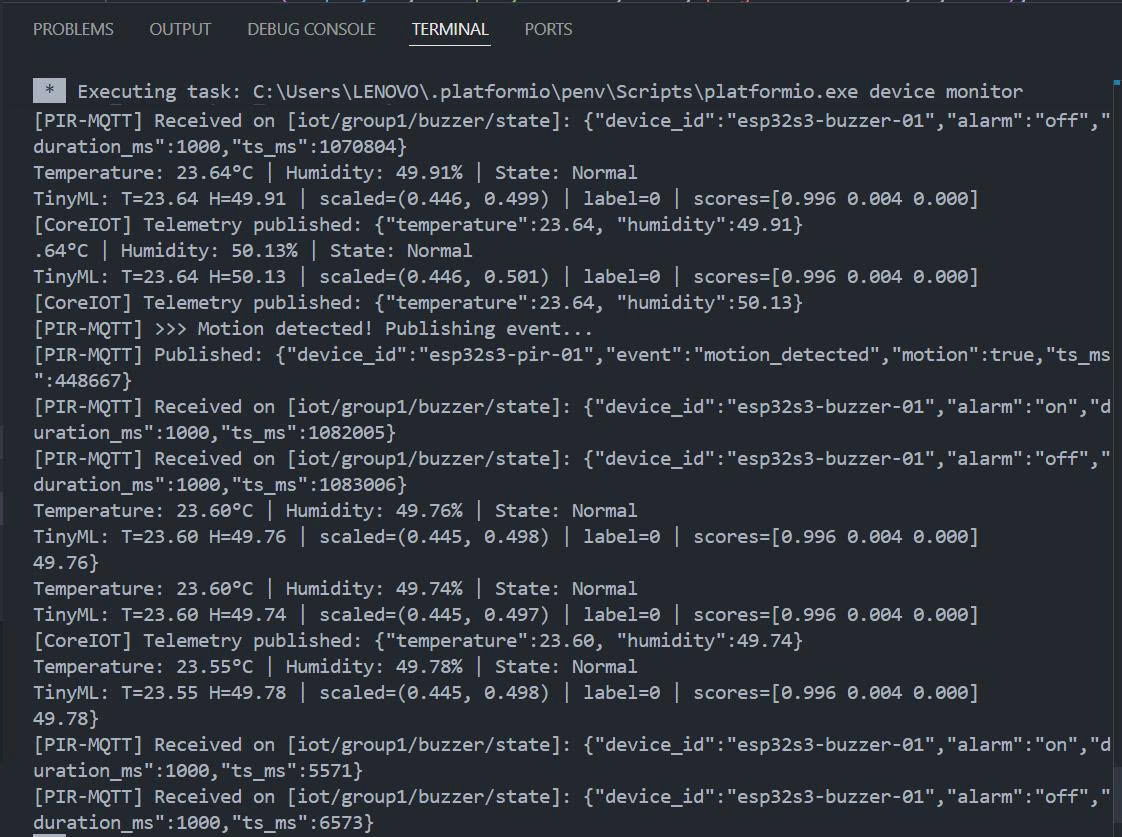
\includegraphics[width=1.1\textwidth]{pictures/res/yolouno_terminal.jpg}
    \caption{Serial Monitor của YoloUNO}
\end{figure}

\begin{figure}[H]
    \centering
    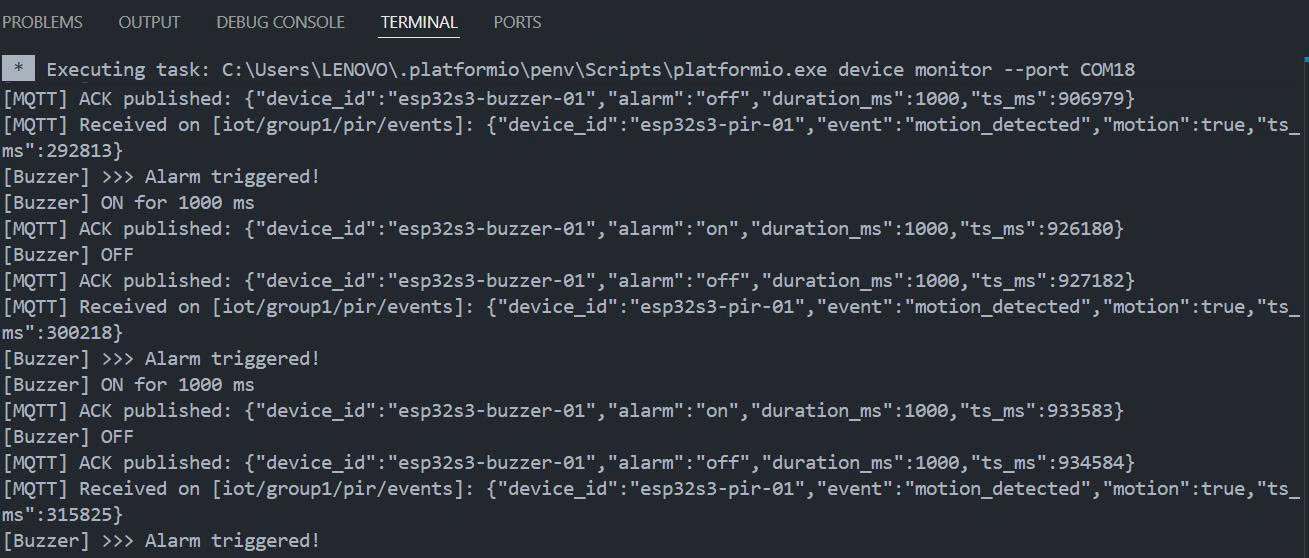
\includegraphics[width=1.1\textwidth]{pictures/res/devkit_terminal.jpg}
    \caption{Serial Monitor của DevKit-C1}
\end{figure}

\subsection{Kết quả kiểm thử chức năng}

\subsubsection*{Task 1 -- LED đơn theo ngưỡng nhiệt độ}

Task 1 hoạt động đúng theo thiết kế 3 vùng nhiệt độ:
\begin{itemize}
    \item $T < 26\,^\circ\mathrm{C}$: LED nháy chậm, độ sáng thấp.
    \item $26 \leq T \leq 28\,^\circ\mathrm{C}$: LED nháy trung bình, độ sáng trung bình.
    \item $T > 28\,^\circ\mathrm{C}$: LED nháy nhanh, độ sáng tối đa.
\end{itemize}
Cơ chế semaphore giữa \texttt{temp\_humi} và \texttt{led\_blinky} cho phản hồi ổn định, không ghi nhận hiện tượng treo hoặc sai trạng thái khi dữ liệu cảm biến thay đổi.

\subsubsection*{Task 2 -- NeoPixel theo độ ẩm và chế độ override}

Task 2 đạt yêu cầu đổi màu theo dải độ ẩm và hoạt động tốt trong cả hai chế độ:
\begin{itemize}
    \item Auto mode: ánh xạ màu Vàng/Xanh lá/Đỏ theo các ngưỡng độ ẩm đã định nghĩa.
    \item Manual override: nhận cờ điều khiển từ cloud để ép LED hiển thị màu Trắng.
\end{itemize}
Trong kiểm thử đa task, việc dùng \texttt{mutex} cho dữ liệu và \texttt{neoPixelMutex} cho phần cứng giúp LED hiển thị ổn định, không bị lỗi nhiễu màu.

\subsubsection*{Task 3 -- Theo dõi nhiệt độ/độ ẩm và hiển thị LCD}

Task 3 đạt yêu cầu cốt lõi:
\begin{itemize}
    \item Đọc DHT20 theo chu kỳ và cập nhật dữ liệu dùng chung.
    \item Kích hoạt semaphore theo ngưỡng trạng thái nhiệt độ.
    \item LCD hiển thị ba trạng thái \texttt{NORMAL / WARNING / CRITICAL} đúng logic.
\end{itemize}

\subsubsection*{Task 4 -- Web server AP/AP+STA và điều khiển thiết bị}

Task 4 hoạt động đúng theo thiết kế:
\begin{itemize}
    \item Thiết bị phát AP để truy cập dashboard cục bộ.
    \item Trang \texttt{/settings} cho phép nhập SSID/password và chuyển sang AP+STA khi kết nối thành công.
    \item API điều khiển LED RGB và quạt phản hồi đúng, trạng thái đồng bộ lại trên giao diện.
\end{itemize}

\subsubsection*{Task 5 -- TinyML trên ESP32-S3}

Kết quả đánh giá mô hình trong phần hiện thực cho thấy:
\begin{itemize}
    \item Mô hình Keras float32 đạt độ chính xác \textbf{1.0000}.
    \item Mô hình TFLite int8 cũng đạt \textbf{1.0000} (360/360 mẫu đúng).
    \item Kết quả trên các kịch bản biên không ghi nhận mẫu phân loại sai.
\end{itemize}
Pipeline huấn luyện, lượng tử hóa và suy luận trên vi điều khiển hoạt động khép kín, đồng bộ qua \texttt{semDataReady} theo đúng thiết kế.

\subsubsection*{Task 6 -- Kết nối cloud CoreIOT}

Task 6 hoạt động ổn định trong các lần thử nghiệm:
\begin{itemize}
    \item Task Wi-Fi tự giám sát và phục hồi kết nối STA khi mất mạng.
    \item Task MQTT publish telemetry định kỳ lên topic chuẩn của CoreIOT.
    \item Cơ chế RPC nhận lệnh từ dashboard và cập nhật cờ override cho Task 1/Task 2 thành công.
\end{itemize}

\subsubsection*{Task mở rộng -- Giao tiếp 2 thiết bị qua Local MQTT}

Kịch bản mở rộng được kiểm thử end-to-end:
\begin{itemize}
    \item PIR node phát hiện chuyển động và publish message lên broker Mosquitto.
    \item Buzzer node subscribe đúng topic, nhận event và kích hoạt còi cảnh báo.
    \item ACK trạng thái buzzer được publish ngược lại phục vụ giám sát/đối soát log.
\end{itemize}

\begin{table}[h!]
\centering
\caption{Tổng hợp test case chính}
\begin{tabular}{|p{3.8cm}|p{4.7cm}|p{4.7cm}|c|}
\hline
\textbf{Hạng mục} & \textbf{Kỳ vọng} & \textbf{Kết quả thực tế} & \textbf{Đánh giá} \\
\hline
Task 1 -- LED theo nhiệt độ & LED có 3 mức hành vi theo ngưỡng nhiệt độ & LED thay đổi đúng tần suất và độ sáng theo từng vùng & Pass \\
\hline
Task 2 -- NeoPixel theo độ ẩm & NeoPixel đổi màu theo 3 dải độ ẩm & Màu sắc phản hồi đúng theo dữ liệu đo & Pass \\
\hline
Task 2 -- Manual override & Bật cờ override thì NeoPixel chuyển trắng & Chuyển trạng thái đúng, không xung đột task & Pass \\
\hline
Task 3 -- State LCD & Hiển thị đúng 3 trạng thái theo ngưỡng nhiệt độ & LCD chuyển trạng thái đúng, có cảnh báo rõ & Pass \\
\hline
Task 4 -- API \texttt{/api/led} & Đổi màu/bật tắt NeoPixel từ web & LED phản hồi theo lệnh, trạng thái đồng bộ & Pass \\
\hline
Task 4 -- API \texttt{/api/fan} & Bật tắt và chỉnh tốc độ quạt & Quạt nhận PWM, thay đổi tốc độ theo slider & Pass \\
\hline
Task 4 -- WiFi settings & Nhập đúng SSID/PASS thì STA kết nối thành công & Thiết bị vào AP+STA, quay về dashboard & Pass \\
\hline
Task 5 -- TinyML accuracy & Độ chính xác suy luận cao, ổn định sau lượng tử hóa & Float32 = 1.0000, Int8 = 1.0000 (360/360) & Pass \\
\hline
Task 6 -- Telemetry/RPC & Publish telemetry và nhận RPC điều khiển từ cloud & Dữ liệu lên dashboard, lệnh RPC xử lý đúng & Pass \\
\hline
MQTT mở rộng & PIR trigger thì buzzer node báo động & Message truyền qua broker, còi kích hoạt đúng & Pass \\
\hline
\end{tabular}
\end{table}

\subsection{Đánh giá tổng quan}

Kết quả thực nghiệm cho thấy hệ thống đạt tính ổn định tốt trong chế độ đa task và đáp ứng đầy đủ các chức năng đã hiện thực trong Chương 4 (Task 1 đến Task 6 và phần mở rộng MQTT liên thiết bị). Kiến trúc dùng semaphore/mutex giúp giảm xung đột tài nguyên, trong khi mô hình MQTT local chứng minh khả năng mở rộng từ một node đơn sang hệ liên thiết bị.

Điểm còn có thể mở rộng ở các vòng sau là bổ sung thêm số đo định lượng (RAM usage, API response time, tỉ lệ reconnect mạng) để tăng chiều sâu phần đánh giá hiệu năng.
